\section{Aufbau und Durchführung}
\label{sec:Durchführung}

\subsection{Elektronische Beschaltung eines Germaniumdetektors}

\begin{figure}
    \centering
    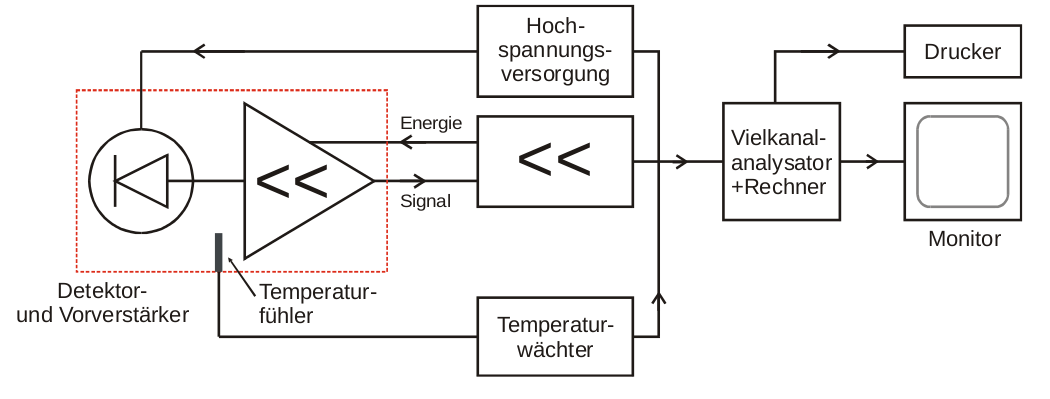
\includegraphics[scale=0.3]{content/aufbau.png}
    \caption{Blockschaltbild des verwendeten Spektrometers [1].}
    \label{fig:aufbau}
\end{figure}


In Abbildung \ref{fig:aufbau} ist das Blockschaltbild und damit der prinzipielle Aufbau des hier verwendeten Germaniumdetektors zu sehen. Ein solcher Detektor ermöglicht es, 
Spannungsimpulse mit einer Höhe proportional zur Gammaquantenenergie zu erzeugen und abzuspeichern. Dazu wird der in der ladungsträgerverarmten Zone erzeugte 
Ladungsimpuls durch elektrische Integration mittels eines kapazitiv gekoppelten Operationsverstärkers in einen Spannungsimpuls umgewandelt. Der Integrationskondensator
wird regelmäßig nach jedem Quantennachweis per optoelektrischer Rückkopplung entladen, da ansonsten das Ausgangspotential des Operationsverstärkers stufenförmig 
ansteigen würde. \\
Die Bandbreite des Verstärkers muss gut angepasst sein, damit keine Rauschspannung entsteht und alle wesentlichen Komponenten des Signals erfasst werden. Dies 
geschieht mittels Hoch- und Tiefpassfiltern. Der Detektor darf nur an die Hochspannung angeschlossen werden, wenn dieser abgekühlt ist. Darum ist ein Temperaturfühler
im Detektorgehäuse eingebaut, der einen Termperaturwächter steuert, sodass die Detektorspannung nicht an einen warmen Kristall gelegt wird. Die Hochspannung 
darf nur langsam geändert werden, da an der Eingangsstufe des Vorverstärkers sonst hohe Spannungen auftreten, die diesen zerstören können. Die Signalspannung wird nun
in einem Vielkanalanalysator gemäß ihrer Höhe in Kanäle einsortiert, welche schließlich auf dem Rechner als Spektrum dargestellt werden. 

\subsection{Messprogramm}

Zur Kalibrierung des Detektors wird das Spektrum von 152-Europium aufgenommen. Aufgrund seiner zahlreichen und bekannten Peaks können mit Hilfe seiner Aktivität $A$
die Effizienz $Q$, sowie die Energiezuordnung der Kanäle berechnet werden. Anschließend wird das Spektrum von 137-Caesium aufgenommen und danach das Spektrum einer
125-Antimon oder einer 133-Barium Quelle. Schließlich wird das Spektrum eines unbekannten Kristalls aufgenommen. 
